\subsection{Background}  
Many people worry about what to wear tomorrow and waste a lot of time trying to find the clothes they want. Moreover, with the improvement of living standards, people pay more attention to how to dress better and how to choose a satisfying outfit according to different needs. To solve these problems, our group come up with an amazing solution, an Intelligent System for Wardrobes.

\subsection{Solution}
To address the problem stated above, we decided to build an intelligent system for the wardrobe. Whenever a user gets new clothes, he/she can register the new clothes by inputting the photo of clothes to our system by phone or pad and it will be labeled automatically (labels could be categories like “jeans” and attributes like “collared”, “woolen”, “red”, etc.). The user can also modify labels if they are not satisfied with them. The system will also allocate a free coat hanger for it and send a message by a Wi-Fi microchip to light up the LED on that coat hanger. After putting the clothes on the hanger, the user can push the button on the hanger to turn off the LED and finish registering. Every day when the user wakes up, he/she can ask our system to recommend what he/she should wear (the decision will be based on criteria like the weather, the place user want to go to, the color matching degree, etc.) After the user become satisfied with a recommended outfit, the LED on the hanger will be lit to help the user find the clothes.

\subsection{Visual Aid}

\begin{figure}[h]
   \centering
   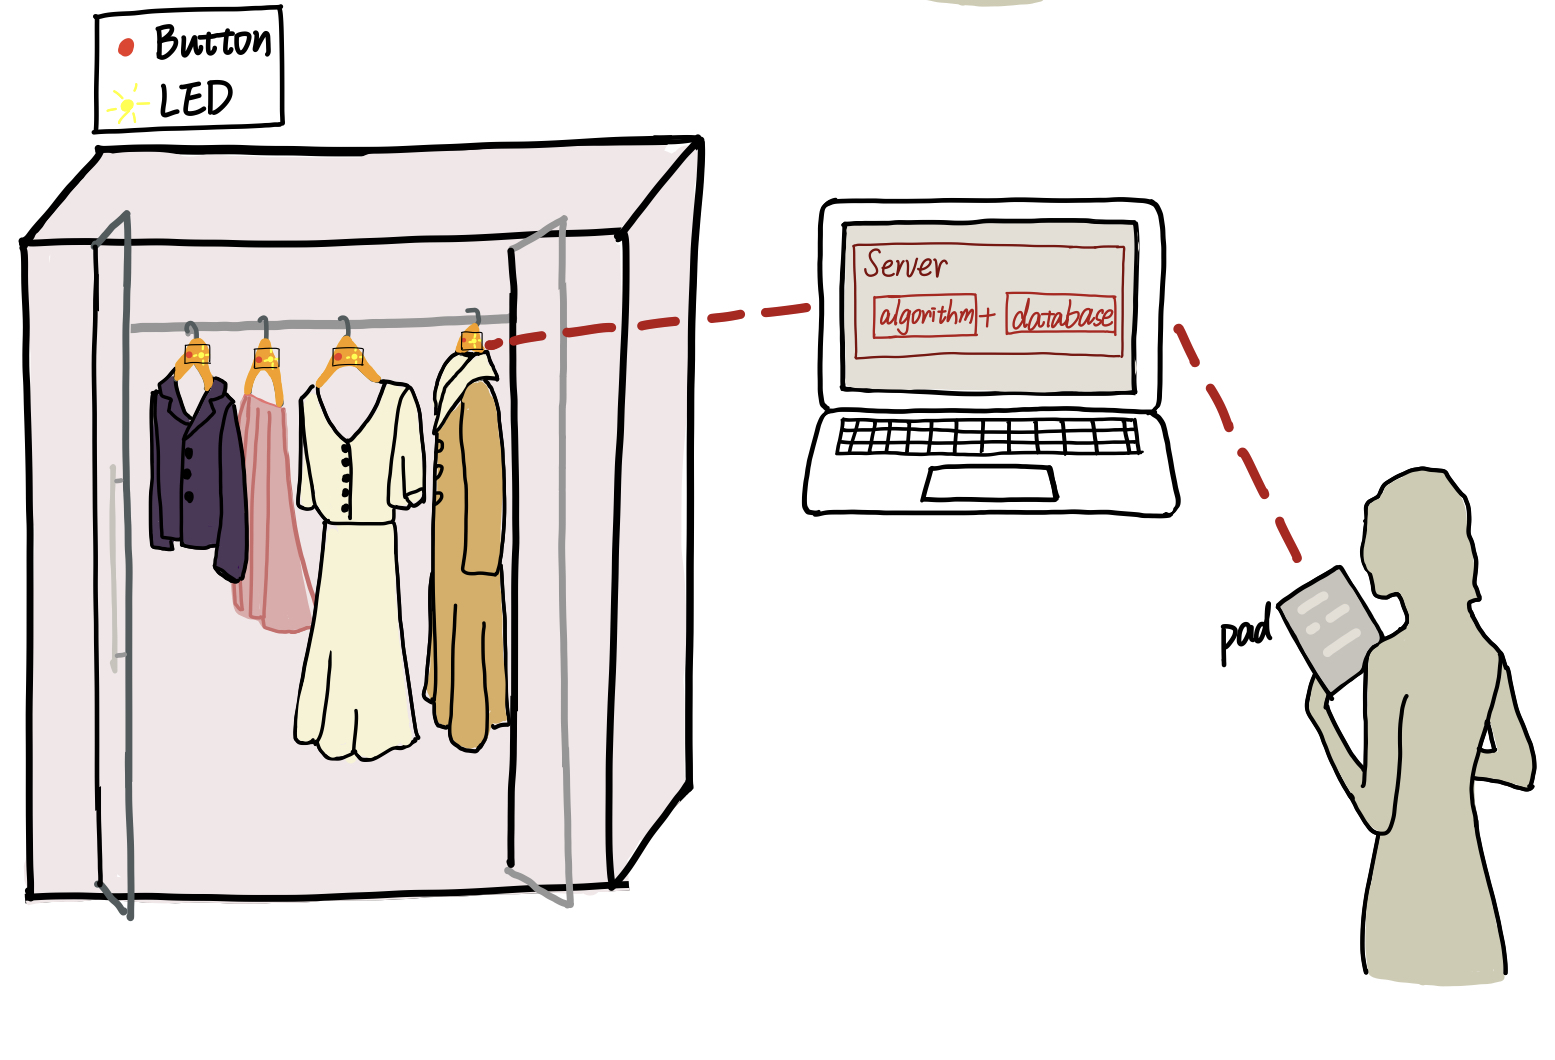
\includegraphics[width=13cm,height=8cm]{graph/physical design.jpg}
   \caption{Physical Design}
   \end{figure}

\subsection{High-level Requirements List}
\begin{itemize}
   \item[$\bullet$] Must recognize the features of the clothes put in with an acceptable accuracy (accuracy \>50\% for category recognition and recall \>30\% for attributes recognition).
   \item[$\bullet$] Must have a usable recommendation function that gives some valuable suggestions (at least 50\% of the recommendations should make sense for at least 50\% test users). Should include some randomness to make the recommendations flexible and allow the unsatisfied users a second chance.
   \item[$\bullet$] Must have a user-friendly interface (at least 80\% test users should find it easy to use). Must allow the users easily and quickly find where the chosen clothes are (the users can find the recommended clothes within 5 seconds).
   \end{itemize}

